\section{Supplementary Tables and Figures for Chapter 2}

\subsection{Supplementary Tables}

\newpage \pdfpagewidth=8.5in \pdfpageheight=16in
\FloatBarrier

\begin{table}
\begin{center}
\begin{tabular}{ccccc}
	Family & Genus & Non-aspirator & Aspirator  & Difference \\
	\midrule
	Neisseriaceae & Neisseria & 7.1 & 41.4 & 34.2 \\
	Porphyromonadaceae & Porphyromonas & 28.6 & 62.1 & 33.5 \\
	Pasteurellaceae & Haemophilus & 50.0 & 82.8 & 32.8 \\
	Lachnospiraceae & Coprococcus & 10.7 & 37.9 & 27.2 \\
	Micrococcaceae & Rothia & 14.3 & 41.4 & 27.1 \\
	Prevotellaceae & Prevotella & 25.0 & 51.7 & 26.7 \\
	Carnobacteriaceae & Granulicatella & 32.1 & 58.6 & 26.5 \\
	Bacillales\_Incertae\_Sedis\_XI & Gemella & 42.9 & 69.0 & 26.1 \\
	Pasteurellaceae & Haemophilus & 57.1 & 82.8 & 25.6 \\
	Actinomycetaceae & Actinomyces & 17.9 & 41.4 & 23.5 \\
	Streptococcaceae & Streptococcus & 39.3 & 62.1 & 22.8 \\
	Lachnospiraceae & Oribacterium & 14.3 & 34.5 & 20.2 \\
	Leptotrichiaceae & Streptobacillus & 17.9 & 37.9 & 20.1 \\
	Lachnospiraceae & Lachnoanaerobaculum & 17.9 & 37.9 & 20.1 \\
	Fusobacteriaceae & Fusobacterium & 42.9 & 62.1 & 19.2 \\
	Prevotellaceae &  & 50.0 & 69.0 & 19.0 \\
	Flavobacteriaceae & Planobacterium & 14.3 & 31.0 & 16.7 \\
	Leptotrichiaceae & Leptotrichia & 14.3 & 31.0 & 16.7 \\
	Erysipelotrichaceae & Solobacterium & 17.9 & 34.5 & 16.6 \\
	Prevotellaceae & Prevotella & 21.4 & 37.9 & 16.5 \\
	Pasteurellaceae & Haemophilus & 28.6 & 44.8 & 16.3 \\
	Veillonellaceae & Veillonella & 35.7 & 51.7 & 16.0 \\
	Prevotellaceae &  & 46.4 & 62.1 & 15.6 \\
	Enterobacteriaceae & Escherichia/Shigella & 46.4 & 62.1 & 15.6 \\
	Neisseriaceae & Neisseria & 60.7 & 75.9 & 15.1 \\
	Streptococcaceae & Streptococcus & 75.0 & 89.7 & 14.7 \\
	Veillonellaceae & Veillonella & 35.7 & 48.3 & 12.6 \\
	Micrococcaceae & Rothia & 42.9 & 55.2 & 12.3 \\
	Streptococcaceae & Streptococcus & 42.9 & 55.2 & 12.3 \\
	Prevotellaceae & Prevotella & 42.9 & 55.2 & 12.3 \\
	Prevotellaceae & Prevotella & 64.3 & 75.9 & 11.6 \\
	Unknown Burkholderiales &  & 10.7 & 20.7 & 10.0 \\
	Bacteroidaceae & Bacteroides & 14.3 & 24.1 & 9.9 \\
	Porphyromonadaceae & Porphyromonas & 21.4 & 31.0 & 9.6 \\
	Moraxellaceae & Moraxella & 39.3 & 48.3 & 9.0 \\
	Prevotellaceae & Prevotella & 57.1 & 65.5 & 8.4 \\
	Leptotrichiaceae & Leptotrichia & 21.4 & 27.6 & 6.2 \\
	Fusobacteriaceae & Fusobacterium & 25.0 & 31.0 & 6.0 \\
	Porphyromonadaceae & Porphyromonas & 50.0 & 55.2 & 5.2 \\
	Neisseriaceae & Neisseria & 17.9 & 20.7 & 2.8 \\
	Veillonellaceae & Veillonella & 89.3 & 89.7 & 0.4 \\
	Unknown Bacteria &  & 21.4 & 20.7 & -0.7 \\
	Coriobacteriaceae & Atopobium & 21.4 & 20.7 & -0.7 \\
	Enterococcaceae &  & 85.7 & 82.8 & -3.0 \\
	Chloroplast & Streptophyta & 10.7 & 6.9 & -3.8 \\
	Pasteurellaceae & Haemophilus & 17.9 & 13.8 & -4.1 \\
	Unknown Bacillales &  & 17.9 & 13.8 & -4.1 \\
	Lactobacillaceae & Lactobacillus & 28.6 & 17.2 & -11.3 \\
	Pasteurellaceae & Haemophilus & 32.1 & 20.7 & -11.5 \\
	Staphylococcaceae & Staphylococcus & 60.7 & 48.3 & -12.4 \\
	Comamonadaceae & Acidovorax & 17.9 & 3.4 & -14.4 \\
	Porphyromonadaceae & Parabacteroides & 21.4 & 6.9 & -14.5 \\
	Comamonadaceae & Pelomonas & 21.4 & 6.9 & -14.5 \\
	Flavobacteriaceae & Chryseobacterium & 28.6 & 13.8 & -14.8 \\
	Erysipelotrichaceae & Clostridium\_XVIII & 21.4 & 3.4 & -18.0 \\
	Lachnospiraceae & Ruminococcus2 & 25.0 & 6.9 & -18.1 \\
	Flavobacteriaceae & Chryseobacterium & 50.0 & 31.0 & -19.0 \\
	Neisseriaceae & Microvirgula & 57.1 & 37.9 & -19.2 \\
	Enterobacteriaceae & Enterobacter & 82.1 & 62.1 & -20.1 \\
	Mycobacteriaceae & Mycobacterium & 28.6 & 6.9 & -21.7 \\
	Moraxellaceae & Acinetobacter & 60.7 & 37.9 & -22.8 \\
	Streptococcaceae & Streptococcus & 60.7 & 37.9 & -22.8 \\
	Bacteroidaceae & Bacteroides & 53.6 & 27.6 & -26.0 \\
	Unknown Bacillales &  & 57.1 & 31.0 & -26.1 \\
	Moraxellaceae & Acinetobacter & 60.7 & 34.5 & -26.2 \\
	Moraxellaceae & Enhydrobacter & 60.7 & 34.5 & -26.2 \\
	Lactobacillaceae & Lactobacillus & 50.0 & 20.7 & -29.3 \\
	Aeromonadaceae & Aeromonas & 57.1 & 27.6 & -29.6 \\
	Moraxellaceae & Acinetobacter & 78.6 & 41.4 & -37.2 \\
	Leuconostocaceae & Leuconostoc & 78.6 & 37.9 & -40.6 \\
	Leuconostocaceae & Weissella & 78.6 & 37.9 & -40.6 \\
	Moraxellaceae & Acinetobacter & 78.6 & 37.9 & -40.6 \\
	Streptococcaceae & Lactococcus & 78.6 & 37.9 & -40.6 \\
	Streptococcaceae & Lactococcus & 78.6 & 37.9 & -40.6 \\
	\bottomrule
\end{tabular}
\caption{Prevalence of lung-gastric fluid exchanged OTUs. Prevalence is calculated as the percentage of patients who have the OTU present in both their lungs and oropharynx, calculated separately among aspirators (N $=$ 29) and non-aspirators (N $=$ 28). OTUs are ordered by their differential prevalence in aspirators relative to non-aspirators, and are labeled with their family- and genus-level taxonomies. Blank genus names indicate OTUs which were not annotated at the genus level.}\label{tab:bal-gastric-exchanged}
\end{center}
\end{table}

\FloatBarrier
\newpage \pdfpagewidth=8.5in \pdfpageheight=11in


%% Classifiers based on abundance of exchanged OTUs
\begin{table}
\begin{center}
%\begin{tabular}{ll}

% Left table - lung-throat
\begin{tabular}{cccc}
\textbf{Lung-oropharynx OTUs (12)} & AUC & p & N (non-asp/asp) \\
\midrule
Lung & 0.60 & 0.32 & 33/33 \\
Oropharyngeal & 0.64 & 0.13 & 43/36 \\
Both & 0.73 & 0.14 & 23/25 \\
\bottomrule
%\end{tabular}
\\
% Right table - lung-gastric
%\begin{tabular}{ccc}
\textbf{Lung-gastric OTUs (75)} &  & & \\
\midrule
Lung & 0.61 & 0.42 & 33/33 \\
Gastric fluid & 0.68 & 0.04 & 48/41 \\
Both & 0.71 & 0.07 & 28/29 \\
\bottomrule
\end{tabular}
%\end{tabular}
\caption{\textbf{Classifiers based on the abundance of exchanged OTUs.} (Top) Classifiers built from the abundance of lung-oropharynx exchanged OTUs. (Bottom) Classifiers built from the abundance of lung-gastric exchanged OTUs. Rows indicate which microbial community was used to train each classifier. In classifiers using two sites (``Both''), abundances of each exchanged OTU in each site were considered as separate features. AUCs are calculated as the area under the average ROC curve from five-fold cross validation. Fisher's exact p values are calculated on the predictions on the hold-out data for all cross validation folds using Python's \texttt{scipy.stats.fisher\_exact} function. Each classifier was built 100 times with random patient splits and classifier initializations, and mean values are reported here. AUCs and Fisher p-values from all 100 repetitions for all classifiers are shown in Supplementary Figures \ref{fig:exchanged_cls_aucs} and \ref{fig:exchanged_cls_p}.)}\label{tab:abun-exchange-classifiers}
\end{center}
\end{table}

\newpage
\FloatBarrier

\subsection{Supplementary Figures}

% Exchange schematic
\begin{figure}[h]
        \begin{center}
        \makebox[\textwidth][c]{\includegraphics[width=\textwidth]{exchange_schematic.png}}
        \caption{Schematic illustrating an OTU which is considered exchanged between the lung and stomach (left) and one which is not (right). If an OTU is exchanged in two sites, its abundance in the two sites should be correlated across patients. Lung image was adapted from Cancer Research UK / Wikimedia Commons and the stomach image from Servier Medical Art.}
        \label{fig:exchanged_schematic}
        \end{center}
\end{figure}


% Exchanged OTUs classifiers (AUCs)
\begin{figure}[h]
        \begin{center}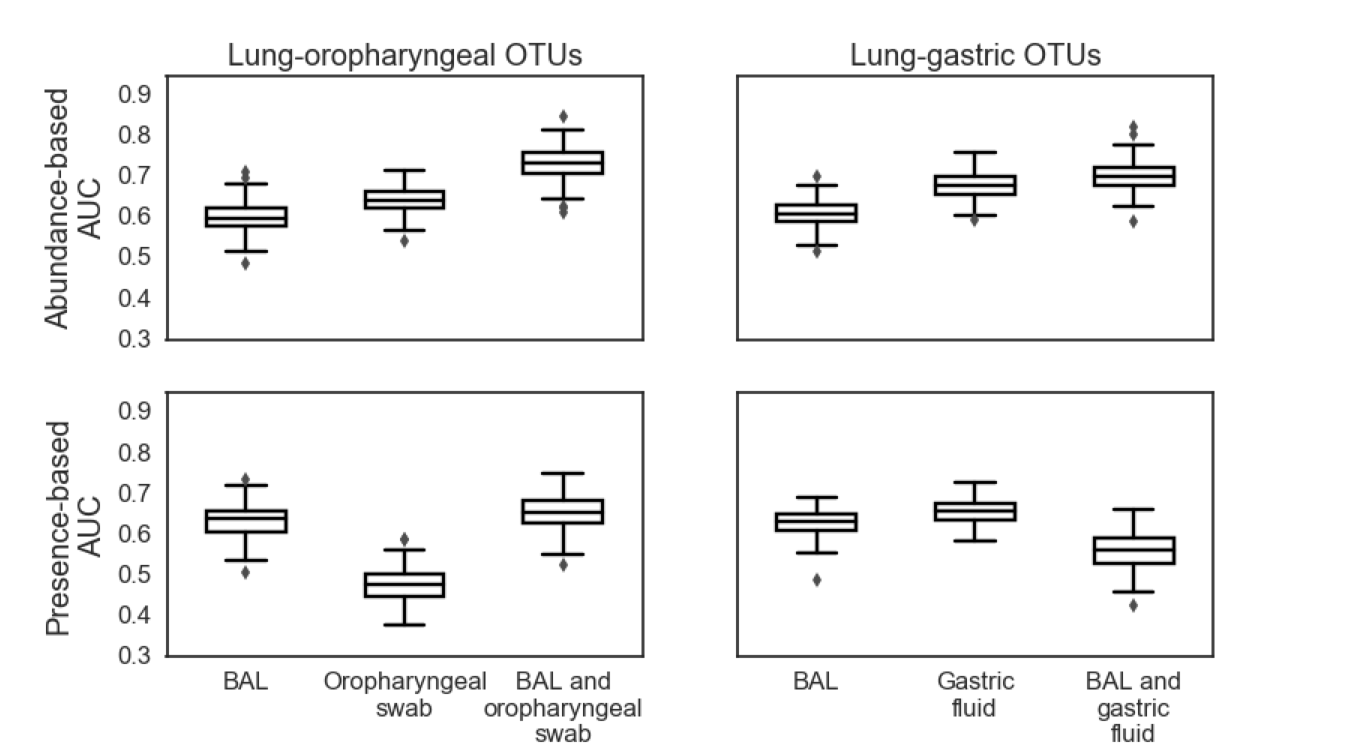
\includegraphics[width=0.8\textwidth]{asp_cls_exchanged_aucs.png}
        \caption{Areas under the ROC curve (AUC) for 100 classifiers trained on the abundance (top) or presence (bottom) of lung-oropharynx exchanged OTUs (left) or lung-gastric exchanged OTUs (right).}
        \label{fig:exchanged_cls_aucs}
        \end{center}
\end{figure}

% Exchanged OTUs classifiers (Fisher p values)
\begin{figure}[h]
        \begin{center}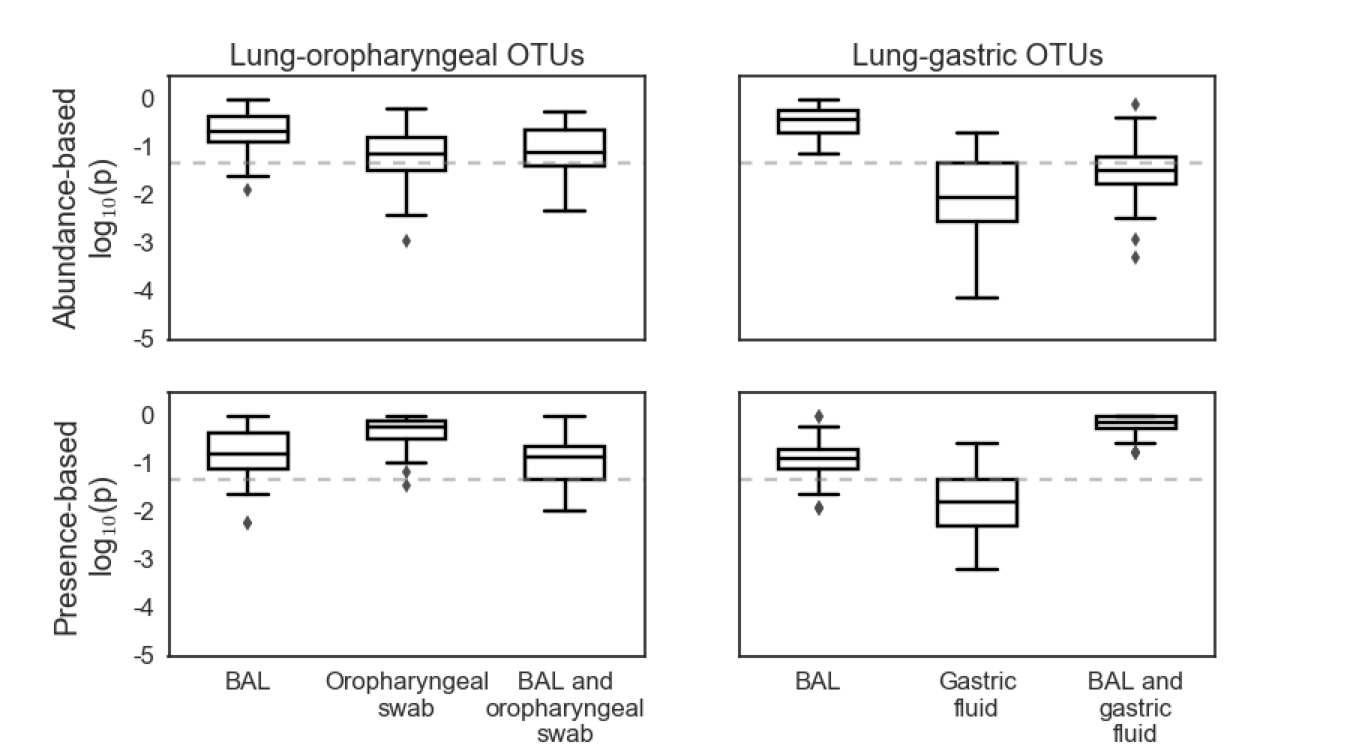
\includegraphics[width=0.8\textwidth]{asp_cls_exchanged_fisherp.png}
        \caption{Log of the Fisher p-values for 100 classifiers trained on the abundance (top) or presence (bottom) of lung-oropharynx exchanged OTUs (left) or lung-gastric exchanged OTUs (right). Dashed line indicates p $=$ 0.05.}
        \label{fig:exchanged_cls_p}
        \end{center}
\end{figure}

% Full community classifiers (AUCs and fisher p values)
\begin{figure}[h]
        \begin{center}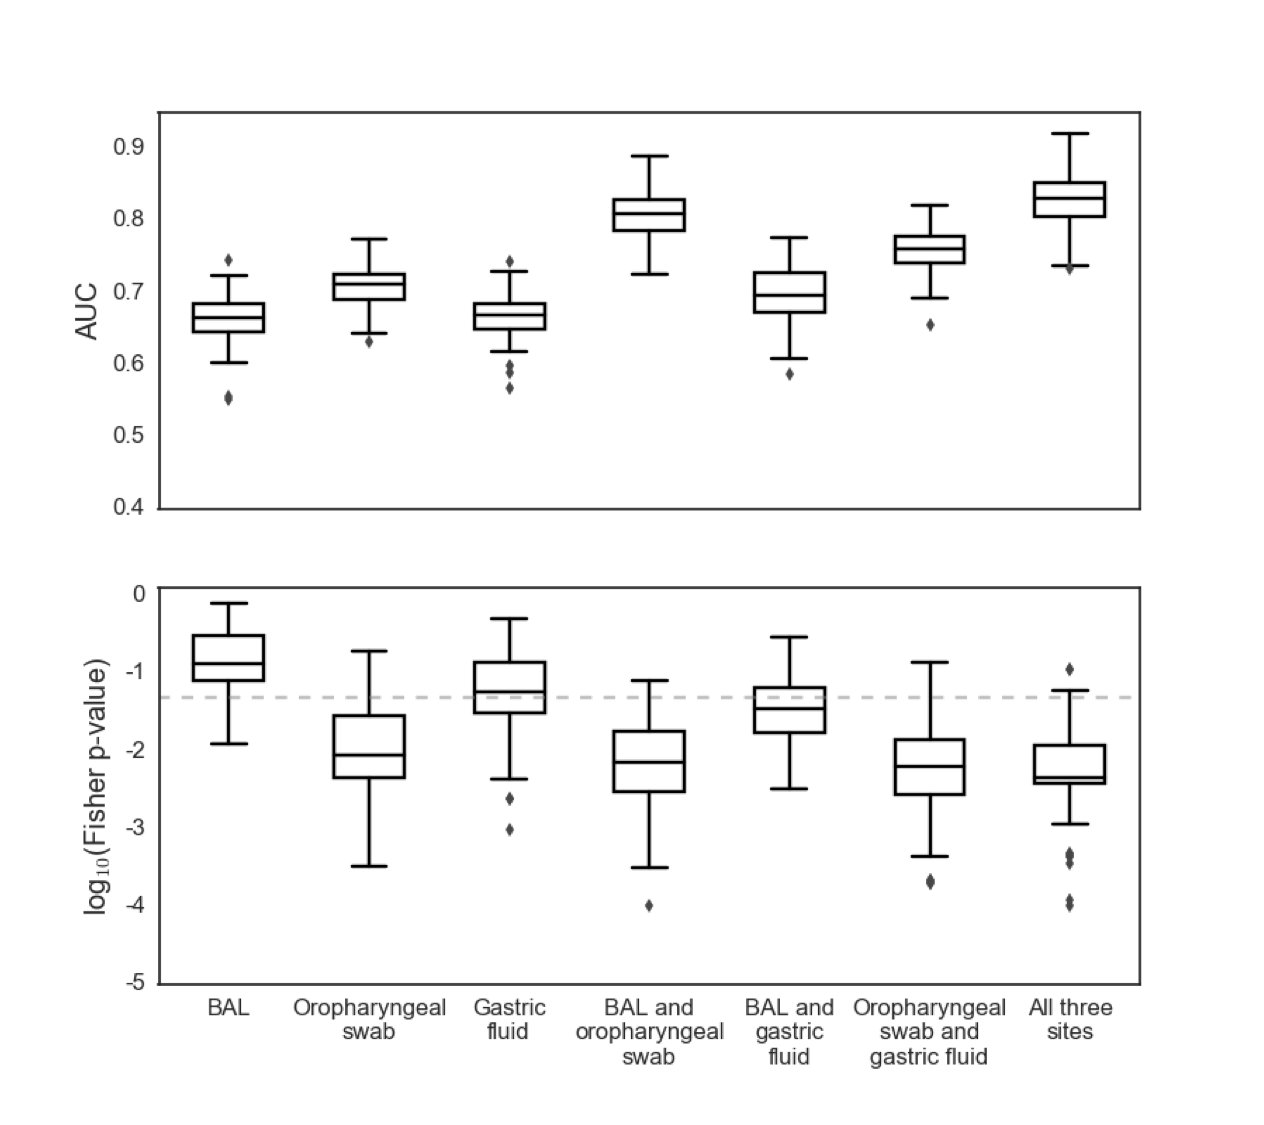
\includegraphics[width=0.8\textwidth]{asp_classifiers_aucs_fisherp.png}
        \caption{Area under the ROC curve (AUC) (top) and Fisher p-values (bottom) for 100 classifiers trained on different combinations of the full aerodigestive communities to distinguish aspirators from non-aspirators. Dashed line on the p value plot is p $=$ 0.05.}
        \label{fig:aucs_pvalues}
        \end{center}
\end{figure}
